% IEEE standard conference template; to be used with:
%   spconf.sty  - LaTeX style file, and
%   IEEEbib.bst - IEEE bibliography style file.
% --------------------------------------------------------------------------

\documentclass[letterpaper]{article}
\usepackage[hidelinks]{hyperref}
\usepackage{spconf,amsmath,amssymb,graphicx}
\usepackage{cleveref}
\usepackage{algorithm}
\usepackage{epstopdf}
\usepackage[font=small,skip=5pt]{caption}
\usepackage{comment}
\usepackage[noend]{algpseudocode}
\usepackage{listings}
\usepackage{color}
 
\definecolor{codegreen}{rgb}{0,0.6,0}
\definecolor{codegray}{rgb}{0.5,0.5,0.5}
\definecolor{codepurple}{rgb}{0.58,0,0.82}
\definecolor{backcolour}{rgb}{0.95,0.95,0.92}
 
\lstdefinestyle{mystyle}{
    backgroundcolor=\color{backcolour},   
    commentstyle=\color{codegreen},
    keywordstyle=\color{magenta},
    numberstyle=\tiny\color{codegray},
    stringstyle=\color{codepurple},
    basicstyle=\scriptsize  ,
    breakatwhitespace=false,         
    breaklines=true,                 
    captionpos=b,                    
    keepspaces=false,                 
    numbers=left,                    
    numbersep=5pt,                  
    showspaces=false,                
    showstringspaces=false,
    showtabs=false,                  
    tabsize=2
}
 
\lstset{style=mystyle}

% Example definitions.
% --------------------
% nice symbols for real and complex numbers
\newcommand{\R}[0]{\mathbb{R}}
\newcommand{\C}[0]{\mathbb{C}}

% bold paragraph titles
\newcommand{\mypar}[1]{{\bf #1.}}

% Title.
% ------
\title{Quantized neural network with four bits compression}
%
% Single address.
% ---------------
\name{Ladislas de Naurois, Matteo Turchetta, Luca Corinzia} 
\address{Department of Computer Science\\ ETH Z\"urich\\Z\"urich, Switzerland}

% For example:
% ------------
%\address{School\\
%		 Department\\
%		 Address}
%
% Two addresses (uncomment and modify for two-address case).
% ----------------------------------------------------------
%\twoauthors
%  {A. Author-one, B. Author-two\sthanks{Thanks to XYZ agency for funding.}}
%		 {School A-B\\
%		 Department A-B\\
%		 Address A-B}
%  {C. Author-three, D. Author-four\sthanks{The fourth author performed the work
%		 while at ...}}
%		 {School C-D\\
%		 Department C-D\\
%		 Address C-D}
%

\begin{document}
%\ninept
%
\maketitle
%

\begin{abstract}
Describe in concise words what you do, why you do it (not necessarily
in this order), and the main result.  The abstract has to be
self-contained and readable for a person in the general area. You
should write the abstract last.
\end{abstract}

\section{Introduction}\label{sec:intro}
In this section we provide a high level overview of the broad impact of neural networks (NNs) across multiple scientific disciplines. We argue about the importance of the performance of forward prediction and finally we discuss previous work that has been done in the field.

%Do not start the introduction with the abstract or a slightly modified
%version. It follows a possible structure of the introduction. 
%Note that the structure can be modified, but the
%%content should be the same. Introduction and abstract should fill at most the first page, better less.
\mypar{Motivation} In recent years we are witnessing an exponential increase in the amount of data available for analysis in almost all scientific disciplines. As a result, there has been a growing interest in machine learning methods to conduct such analysis. Among these, Neural Networks (NNs) are regarded as one of the most promising techniques. 
They have been successfully applied to a wide range of tasks (often outperforming the state of the art) including medical applications \cite{amato_artificial_2013}, image recognition \cite{krizhevsky_imagenet_2012} and robotics \cite{gu_deep_2016}. 

One of the main drawbacks of NNs is that they make use of a high number of parameters. This means that the network requires a lot of memory resources for storage and a lot of computational resources for training and forward prediction. While the training phase usually is performed on powerful parallel computing architectures where there is an abundance of both computational and memory resources, the platforms that make use of the trained network usually have much more limited capabilities (e.g. mobile phones). This problem has steered attention of the research community toward reducing the memory and computation requirements for trained NNs.

A promising direction along this line of research is known as quantized neural networks (QNNs). The central idea to QNNs is to compress the parameters of the network from their float representation to a light-weight one based on quantization bins. The parameter space is divided into a predefined number of bins and each parameter value 
 The first task is to motivate what you do.  You can
start general and zoom in one the specific problem you consider.  In
the process you should have explained to the reader: what you are doing,
why you are doing, why it is important (order is usually reversed).

For example, if my result is the fastest DFT implementation ever, one
could roughly go as follows. First explain why the DFT is important
(used everywhere with a few examples) and why performance matters (large datasets,
realtime). Then explain that fast implementations are very hard and
expensive to get (memory hierarchy, vector, parallel). 

Now you state what you do in this paper. In our example: 
presenting a DFT implementation that is
faster for some sizes than all the other ones.

\mypar{Related work} Next, you have to give a brief overview of
related work. For a paper like this, anywhere between 2 and 8
references. Briefly explain what they do. In the end contrast to what
you do to make now precisely clear what your contribution is.

\section{Background: NNs and QNNs}\label{sec:background}

In this section we formally introduce NNs and QNNs and relative notation.

\mypar{Artificial neural networks}
An artificial neural network (NN) is non linear map from an input vector $\mathbf{x} \ \in \mathbb{R}^{d_i}$ to an output vector $f(\mathbf{x} ) = \mathbf{y} \ \in \mathbb{R}^{d_o}$. A one-layer NN implements this mapping by composing a linear transformation $ \mathbf{a} = \mathbf{W}\mathbf{x} + \mathbf{b}$ with a non linear one $\mathbf{y} = \phi(\mathbf{a})=\phi(\mathbf{W}\mathbf{x} + \mathbf{b})$.  The matrix $\mathbf{W}$ is called \emph{weight matrix}, the vector $\mathbf{b}$ is called \emph{bias vector} and the non-linear transformation $\phi(\cdot)$ is called \emph{activation function}. In a multi layer NN the mapping $f$ is implemented by composing a sequence such layers, i.e. by feeding the output of a layer as input to the subsequent one:
\begin{equation}\label{eq:deepNN}
\mathbf{y} =\phi_1(\mathbf{W_1}\mathbf{\phi_2(\mathbf{W_2}\phi_3(\mathbf{\cdots}) + \mathbf{b_2})} + \mathbf{b_1}).
\end{equation}
% The map $f$ is built recursively applying at step $t$ a linear transformation $ \mathbf{a}_t = \mathbf{W}_t\mathbf{x}_t + \mathbf{b}_t$ and a non-linear transformation $\mathbf{x}_{t+1} = \phi_t(\mathbf{a}_t)$. The matrix $\mathbf{W}_t$ is called \emph{weight matrix}, and the vector $\mathbf{b}_t$ is called \emph{bias vector}. The step $t$ is also know as the \emph{layer} index. 

\mypar{Quantized neural network}
A quantized neural network (QNN) is a NN that uses low precision weight matrix and bias vector. Formally, given a one-layer NN with parameters $\{\mathbf{W}\}, \{\mathbf{b}\}$ and activation functions $\phi(\cdot)$, its quantized implementation applies  the linear transformation $\mathbf{a} = \mathcal{Q}(\mathbf{W}) \mathcal{Q}(\mathbf{x}) + \mathcal{Q}(\mathbf{b})$ and the non-linear transformation $\mathbf{y} = \phi(\mathbf{a})$, where $\mathcal{Q}(\cdot)$ is the quantization function that we introduce in the following section. Similarly to the standard case, multi-layer QNNs are implemented by composition of individual layers as in \cref{eq:deepNN}.

\mypar{Matrix quantization} For a matrix $\mathbf{A}$, the function $\mathcal{Q}(\mathbf{A})$ returns a low precision encoding of the matrix $\mathbf{A}$. It first computes the minimum entry ($mn$) and the maximum entry ($mx$) of the matrix $\mathbf{A}$. Then, given $k$ bits it builds a linear binning of the continuous interval $[mn,mx]$ into $2^k$ bins. The bin size of the quantization $\Delta(\mathbf{A})$ is then \[\Delta(\mathbf{A}) = \frac{mx - mn}{2^k}\] To insure that the value $0$ is represented exactly as a bin value, its index is computed as \[z(\mathbf{A}) = sat([-mn/\Delta(\mathbf{A})])\] where the brackets $[\cdot]$ stand for the rounding to the closest integer and the $sat(\cdot)$ function saturates an integer value into the integer value representable with k bits, hence it reads $sat(n) = \max(0, \min(n,2^k) )$. The bin values are then $\{ (i-z(\mathbf{A})) \Delta(\mathbf{A}), \ \ i = 0, \dots, 2^k -1 \}$. Then every entry $A_{ij}$ is quantized to the closest bin value. The quantize matrix  $\mathcal{Q}(\mathbf{A})$ and the quantized integer matrix $\tilde{\mathcal{Q}}(\mathbf{A})$ have respectively the bin value and the bin index as their $ij$ entry. Note that the matrix $\mathcal{Q}(\mathbf{A})$ is a real-valued matrix, while $\tilde{\mathcal{Q}}(\mathbf{A})$ is k-bit integer valued, and also that the following holds:
\begin{equation}\label{equation:affine_transf}
\mathcal{Q}(\mathbf{A}) = (\tilde{\mathcal{Q}}(\mathbf{A}) -z(\mathbf{A}) \mathbf{J}  ) \Delta(\mathbf{A})
\end{equation} 
where $\mathbf{J}$ is a matrix with all entries equal to one. The algorithm to compute $\tilde{\mathcal{Q}}(\mathbf{A})$  is showed in \cref{algorithm:quantize}.

\begin{algorithm}
	\caption{Quantize}\label{algorithm:quantize}
	\begin{algorithmic}[1]
		\State compute $mn = \min A_{ij}$ and $mx = \max A_{ij}$
		\State $\Delta = \frac{mx - mn}{2^k}$.
		\State $z = -mn/\Delta$
		\For{$i,j = 1, \dots N$}
			\State $\tilde{\mathcal{Q}}(\mathbf{A})_{ij} = saturate([A_{ij}/\Delta + z ])$ 
		\EndFor
	\end{algorithmic}
\end{algorithm}

\mypar{Quantized Matrix-Matrix Multiplication} Given two matrices $\mathbf{L}$ and $\mathbf{R}$, we want to compute the product $\mathcal{Q}(\mathbf{L}) \mathcal{Q}(\mathbf{R})$. Using \cref{equation:affine_transf} and we write the product as 
\begin{align}\label{equation:qmmm}
\begin{split}
& \mathcal{Q}(\mathbf{L}) \mathcal{Q}(\mathbf{R}) =\\
 & \Delta (\mathbf{L})\left( \tilde{\mathcal{Q}}(\mathbf{L}) - z(\mathbf{L})\mathbf{J} \right)
\left( \tilde{\mathcal{Q}}(\mathbf{R}) - z(\mathbf{R})\mathbf{J} \right)  \Delta (\mathbf{R}).
\end{split}
\end{align}
Inverting the equation \ref{equation:affine_transf}  we can then obtain the k-bit integer valued product matrix as 
\begin{equation}\label{equation:affine_inverse}
\tilde{\mathcal{Q}}(\mathbf{LR}) = sat([\frac{1}{\Delta(\mathbf{LR})}\mathcal{Q}(\mathbf{L}) \mathcal{Q}(\mathbf{R}) + z(\mathbf{LR}) \mathbf{J}])
\end{equation} The algorithm for Quantized Matrix Matrix Multiplication (QMMM) is shown in \cref{algorithm:qmmm}.

\begin{algorithm}
	\caption{QMMM}\label{algorithm:qmmm}
	\begin{algorithmic}[1]
		\State compute $\mathcal{Q}(\mathbf{L}) \mathcal{Q}(\mathbf{R})$ as in \cref{equation:qmmm}
		\State compute the k-bit integer matrix $\tilde{\mathcal{Q}}(\mathbf{LR})$ as in \cref{equation:affine_inverse}
 	\end{algorithmic}
\end{algorithm}


\section{Your Proposed Method}\label{sec:yourmethod}
In this section we propose an optimized implementation of the quantization and Quantized Matrix-Matrix Multiplication (QMMM) functions introduced in \cref{sec:background} that uses four bits compression. We start by presenting the data structure that we use for our baseline implementation. We continue by analysing the bottlenecks of this implementation and by proposing a set of solutions to achieve a higher performance.

\mypar{Baseline implementation}
We presented the algorithm at the base of a straight forward implementation of a simple QNN using a $k$-bits compression scheme in \cref{sec:background}. Here we introduce the data structure necessary to a naive implementation in case $k=4$. Using a 4-bits compression scheme presents challenges due to the byte addressability of the computer memory and to the lack of a built-in 4-bits integer data type. As a consequence, we have to define our custom data structure. One way of operating on entities that require less than a byte for storage is to use structs in combination with bit fields. Nevertheless, byte addressability of the memory does not make it possible to load or store less than one byte at a time. Hence, using bit fields to define a custom data type that stores a single 4-bits integer is wasteful.  In the proposed solution we define the $uint4x4_t$ data structure. This is a 2 bytes struct that exploits bit fields to store four integers of 4 bits each. The reason why we pack four integers in one struct instead of two is because it allows us to define a data type that is more convenient for QMMM. In particular, one $uint4x4_t$


Our baseline implementation consists of two parts:
\begin{itemize}
\item Scalar quantization
\item Scalar matrix to matrix multiplication
\end{itemize}

\textbf{Scalar Quantization: } Our input data \emph{v} is a vector of 32-bit floats that contains the values for an arbitrary matrix of size $\emph{rows} \times \emph{columns} \in \mathbb{N} \times \mathbb{N} $, i.e.\ $ \emph{v} \in \mathbb{R}^{ \emph{rows} \cdot \emph{columns} } \cong \mathbb{R}^{ \emph{rows} \times \emph{columns} } $. We traverse the values in \emph{v} to identify the minimum (\emph{min}) and maximum (\emph{max}) of the vector, i.e. $ \emph{min} = \min_{ i \in \emph{rows} \cdot \emph{columns} } v[i] , \emph{max} = \max_{i \in \emph{rows} \cdot \emph{columns} } v[i] $. Subsequently, given a desired precision $ \emph{p} \in \mathbb{N} $, we compute the size of a cell in our range $[\emph{min},\emph{max}] \subset \mathbb{R}$ via $ \Delta = \frac{ \emph{max} - \emph{min} }{ 2^{\emph{p}}} \in \mathbb{R} $. Finally, due to the importance of the 0 value in Neural Networks, we apply a correction value to ensure that the 0 value is encoded exactly, computed via $ \zeta = \frac{ | min | }{ \Delta } - \lfloor \frac{ | min | }{ \Delta } \rfloor $. Finally, we may encode every value in \emph{v} according to the encoding scheme: $ \emph{q}[i] = \frac{ \emph{v}[i] } {\Delta} + \zeta , i \in [0, \emph{rows}\cdot\emph{columns}] \cap \mathbb{N} $.

\textbf{Scalar matrix to matrix multiplication: } Once the parameter matrix has been quantized, we arrive at a quantized vector $ \emph{q} \in  \left([0, 2^{\emph{p}} - 1]\right)^{ \emph{rows} \cdot \emph{columns} }$. Assuming that our input vectors ($ \emph{x} \in \mathbb{R}^{rows} $), we must now compute $ \emph{q} \emph{x} $. Given that $ \emph{q} = ( \frac{ \emph{v}[i] }{ \Delta} + \zeta )_{i \in \emph{rows}\cdot\emph{columns}} \cdot \emph{x} = \frac{1}{\Delta} \left(  \emph[v] \cdot \emph{x} \right) + \zeta \cdot (1,1,1,...,1,1) $. Moreover, assuming that the input vectors are encoded in compressed format ($\widetilde{{x}}$), we may rearrange the terms as follows: 
$ \widetilde{{x}}^{T} \cdot \emph{q} = \frac	{1}{\Delta_q \cdot \Delta_x} \left( \emph{x}' \cdot \emph{v} ) + \frac{\zeta_q}{\Delta_x} \emph{x} + \frac{\zeta_x}{\Delta_q} \emph{v} + \zeta_q \cdot \zeta_x \cdot (1,1,1,...,1,1) \right)$.

%Now comes the ``beef'' of the paper, where you explain what you
%did. Again, organize it in paragraphs with titles. As in every section
%you start with a very brief overview of the section.
%
%For this class, explain all the optimizations you performed. This mean, you first very briefly
%explain the baseline implementation, then go through locality and other optimizations, and finally SSE (every project will be slightly different of course). Show or mention relevant analysis or assumptions. A few examples: 1) Profiling may lead you to optimize one part first; 2) bandwidth plus data transfer analysis may show that it is memory bound; 3) it may be too hard to implement the algorithm in full generality: make assumptions and state them (e.g., we assume $n$ is divisible by 4; or, we consider only one type of input image); 4) explain how certain data accesses have poor locality. Generally, any type of analysis adds value to your work.
%
%As important as the final results is to show that you took a structured, organized approach to the optimization and that you explain why you did what you did.
%
%
%Mention and cite any external resources including library or other code.
%
%Good visuals or even brief code snippets to illustrate what you did are good. Pasting large amounts of code to fill the space is not good.

\section{Experimental Results}\label{sec:exp}
\graphicspath{{../../plots/}}
\epstopdfsetup{outdir=./figures/}

In this section we perform the empirical evaluation of the optimization performed as outlined in the \cref{sec:yourmethod}. Every code version is tested for correctness on a small size example with hand-computed output and on several large-size random instances with output given by the naive implementation.

\mypar{Experimental setup}
For the empirical evaluation of the code, we use an Skylake processor (3.5 GHz, L1 cache 128 KB, L2 cache 1 MB, L3 cache 6 Mb). The compiler used is g++ with flags "-O3 -fno-tree-vectorize -march=native -mavx". The matrix size varies in the range $[30,1000]$.

\mypar{Results: operational count optimization}
We first evaluate the gain the in the runtime regarding the optimization in the operational count performed with the trick as in \cref{equation:qmmm_smart}. From \cref{figure:performance_qmm_kernel} we can see the decrease in performance of the trick version with respect to the naive implementation. \cref{figure:cycles_qmm_comparison} shows that the operation count optimization gives an overall speed-up of $15 \%$. In \cref{figure:Cycles_trick} we can see the contribution of each function of the pipeline in the overall runtime. In the following the trick version is further optimized.

\begin{figure}[h]
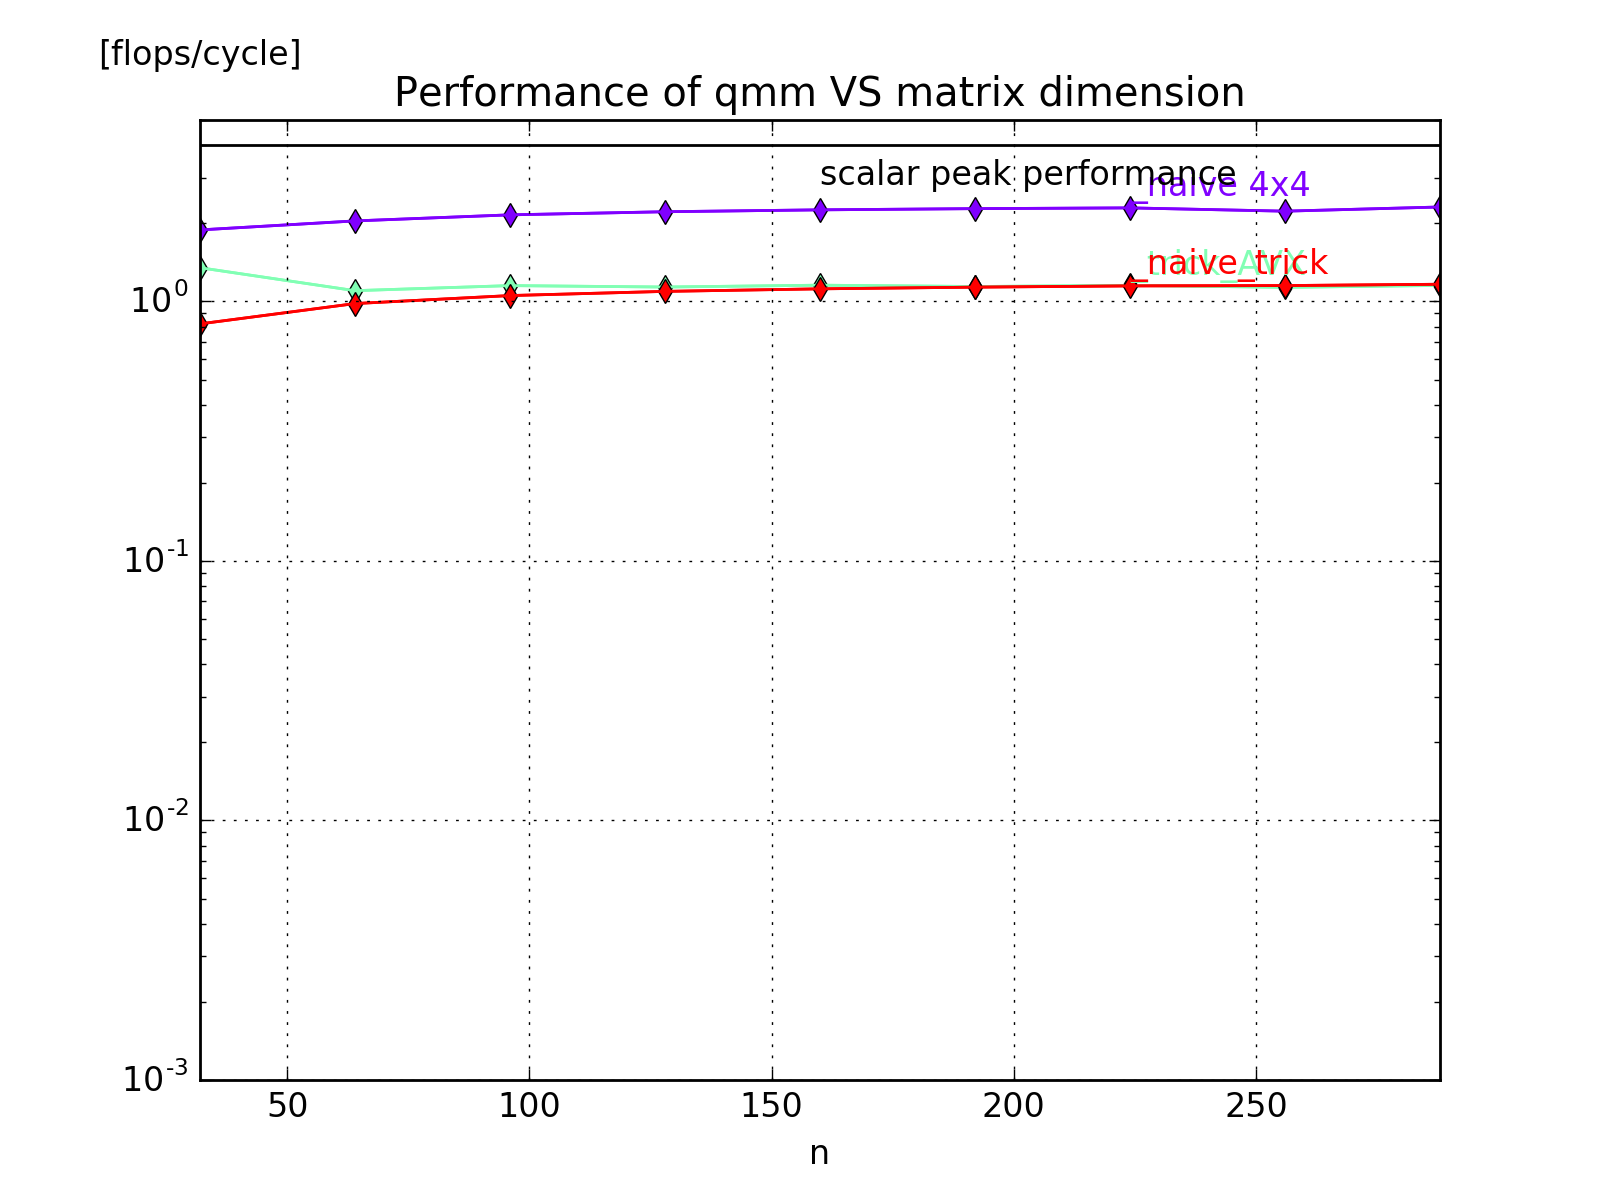
\includegraphics[width=0.5\textwidth]{Performance_qmm.eps}
\caption{Performance plot for the QMM kernel}
\label{figure:performance_qmm_kernel}
\end{figure}

\begin{figure}[h]
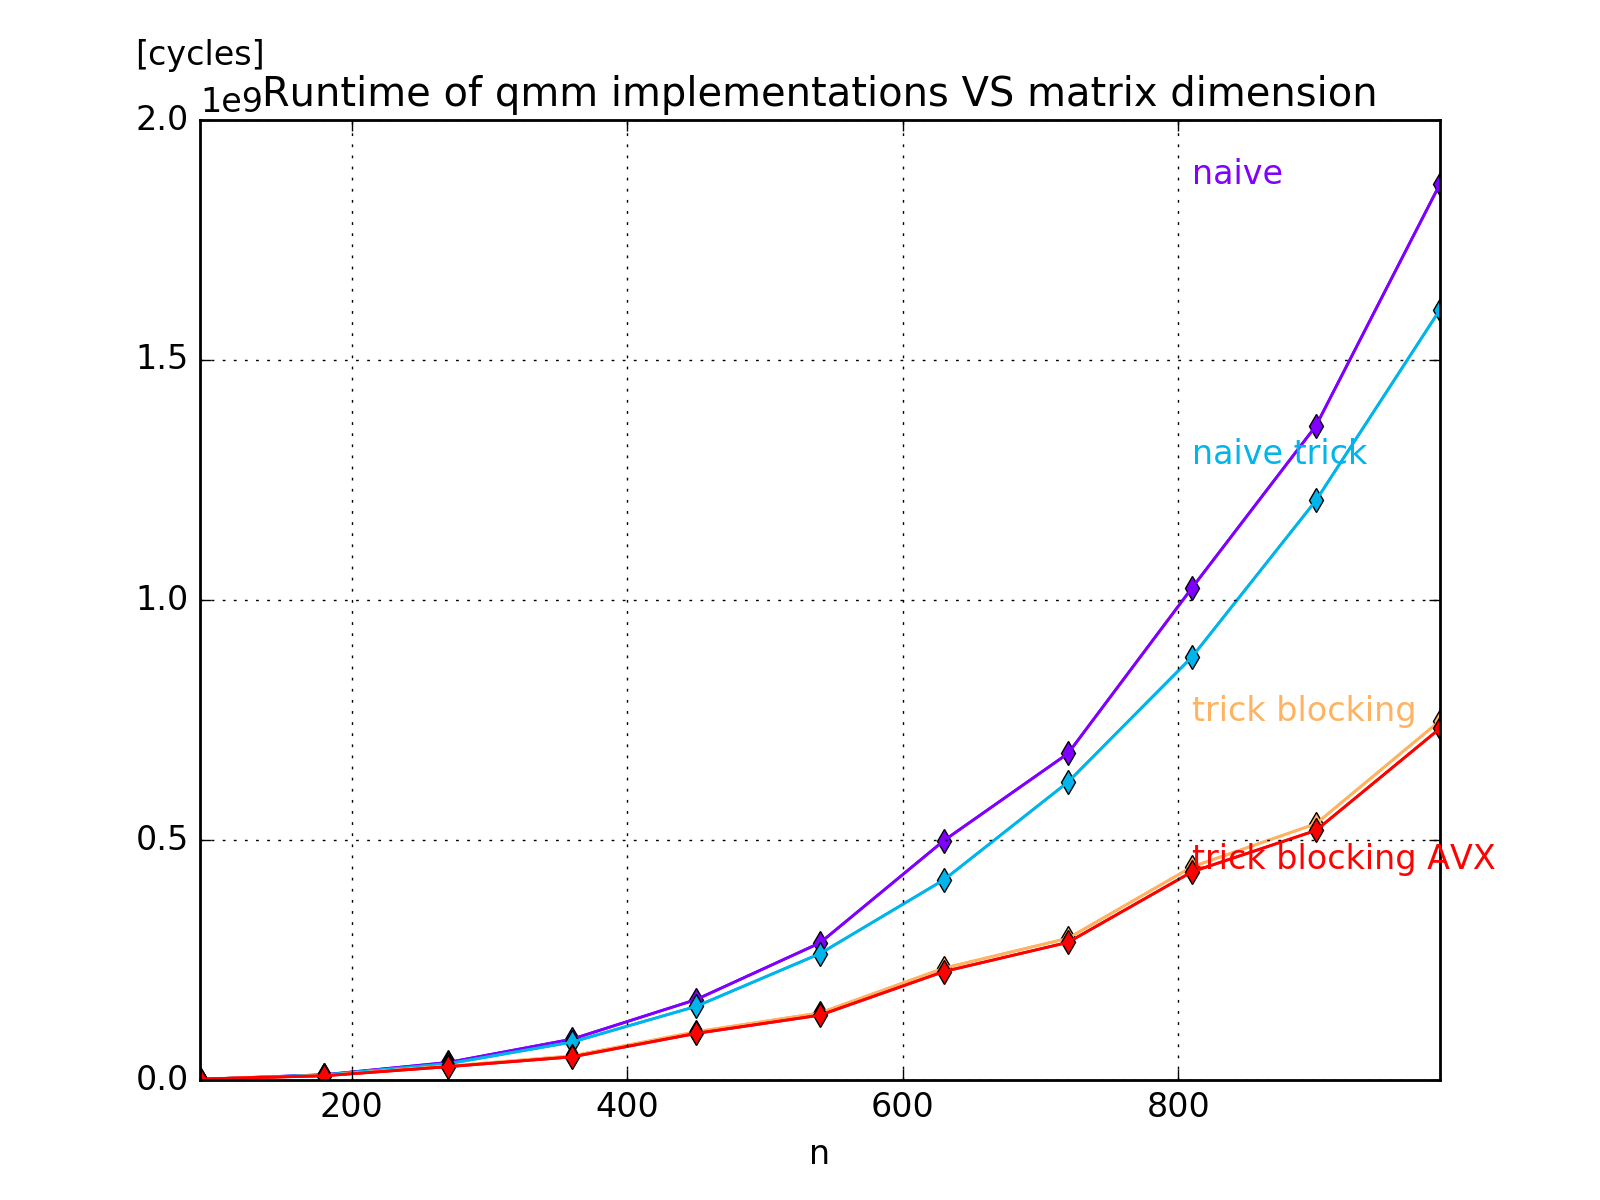
\includegraphics[width=0.5\textwidth]{Cycles_qmm_comparison.eps}
\caption{Runtime plot of the overall pipeline}
\label{figure:cycles_qmm_comparison}
\end{figure}

\begin{figure}[h]
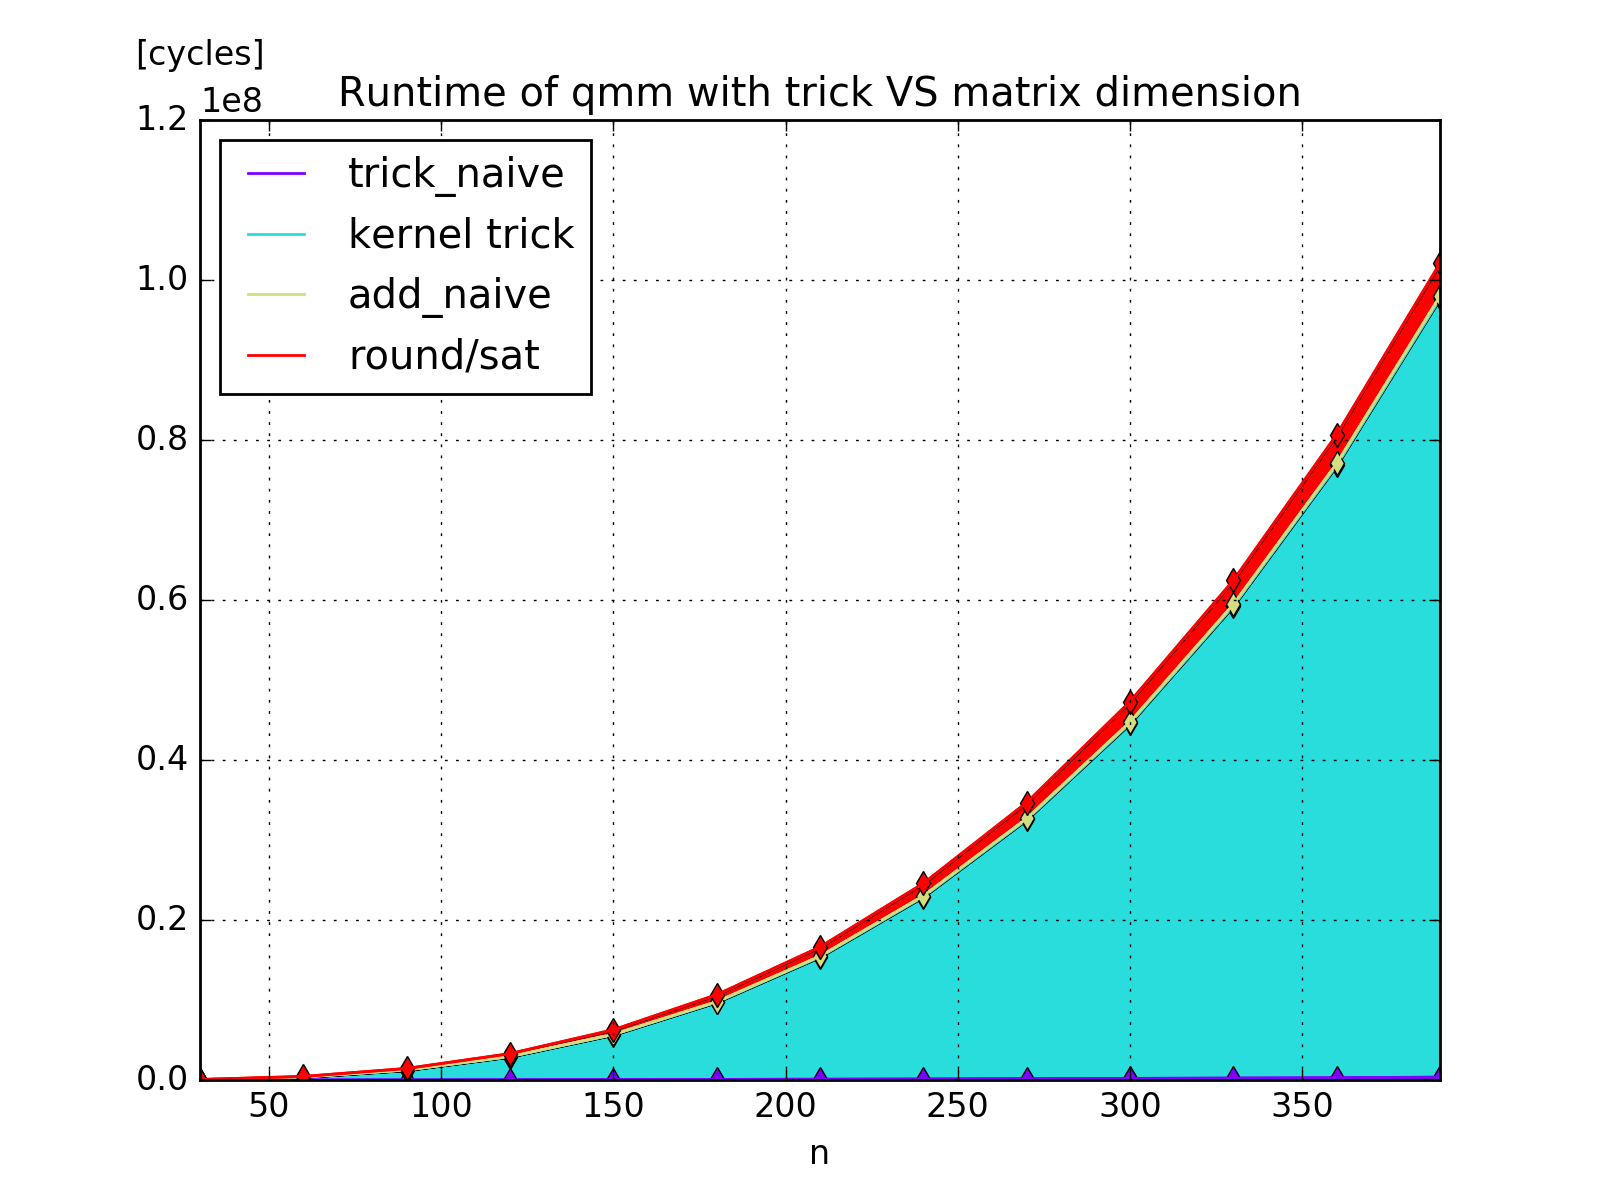
\includegraphics[width=0.5\textwidth]{Cycles_trick.eps}
\caption{Contribution of each naive-version sub-function in the overall runtime.} 
\label{figure:Cycles_trick}
\end{figure}


\mypar{Results: blocking for MMM}
The blocking parameter used is $N_b = 30$ for the cache blocking parameter and $n_b = 3$ for the register blocking parameter, as described in \cref{sec:yourmethod}. \cref{figure:performance_qmm_kernel} shows the gain in performance with respect to the naive\_trick implementation. The large $n$ performance gain is approximately $2$X. Note that the blocking parameter for cache and for register are not fine tuned, so a further speedup could be possible.


\mypar{Results: vectorization} 
In this paragraph we evaluate the performance gain thanks to vectorization for \emph{trick\_vector}, \emph{quantize}, \emph{add\_trick\_vector} and \emph{round\_saturation} as outlined in \cref{sec:yourmethod}. \cref{figure:performance_add_vector} and \cref{figure:performance_trick_vector} show a linear increase of the performance for small instances. This is due to a border effect. The instance size in the  performance plot are not in general a multiple of the vector size ($16$X$16 \ Bits$), hence for small instance size the scalar computation can be non-negligible. Moreover the scalar contribution decreases linearly with the size of the instance.

\begin{figure}[h]
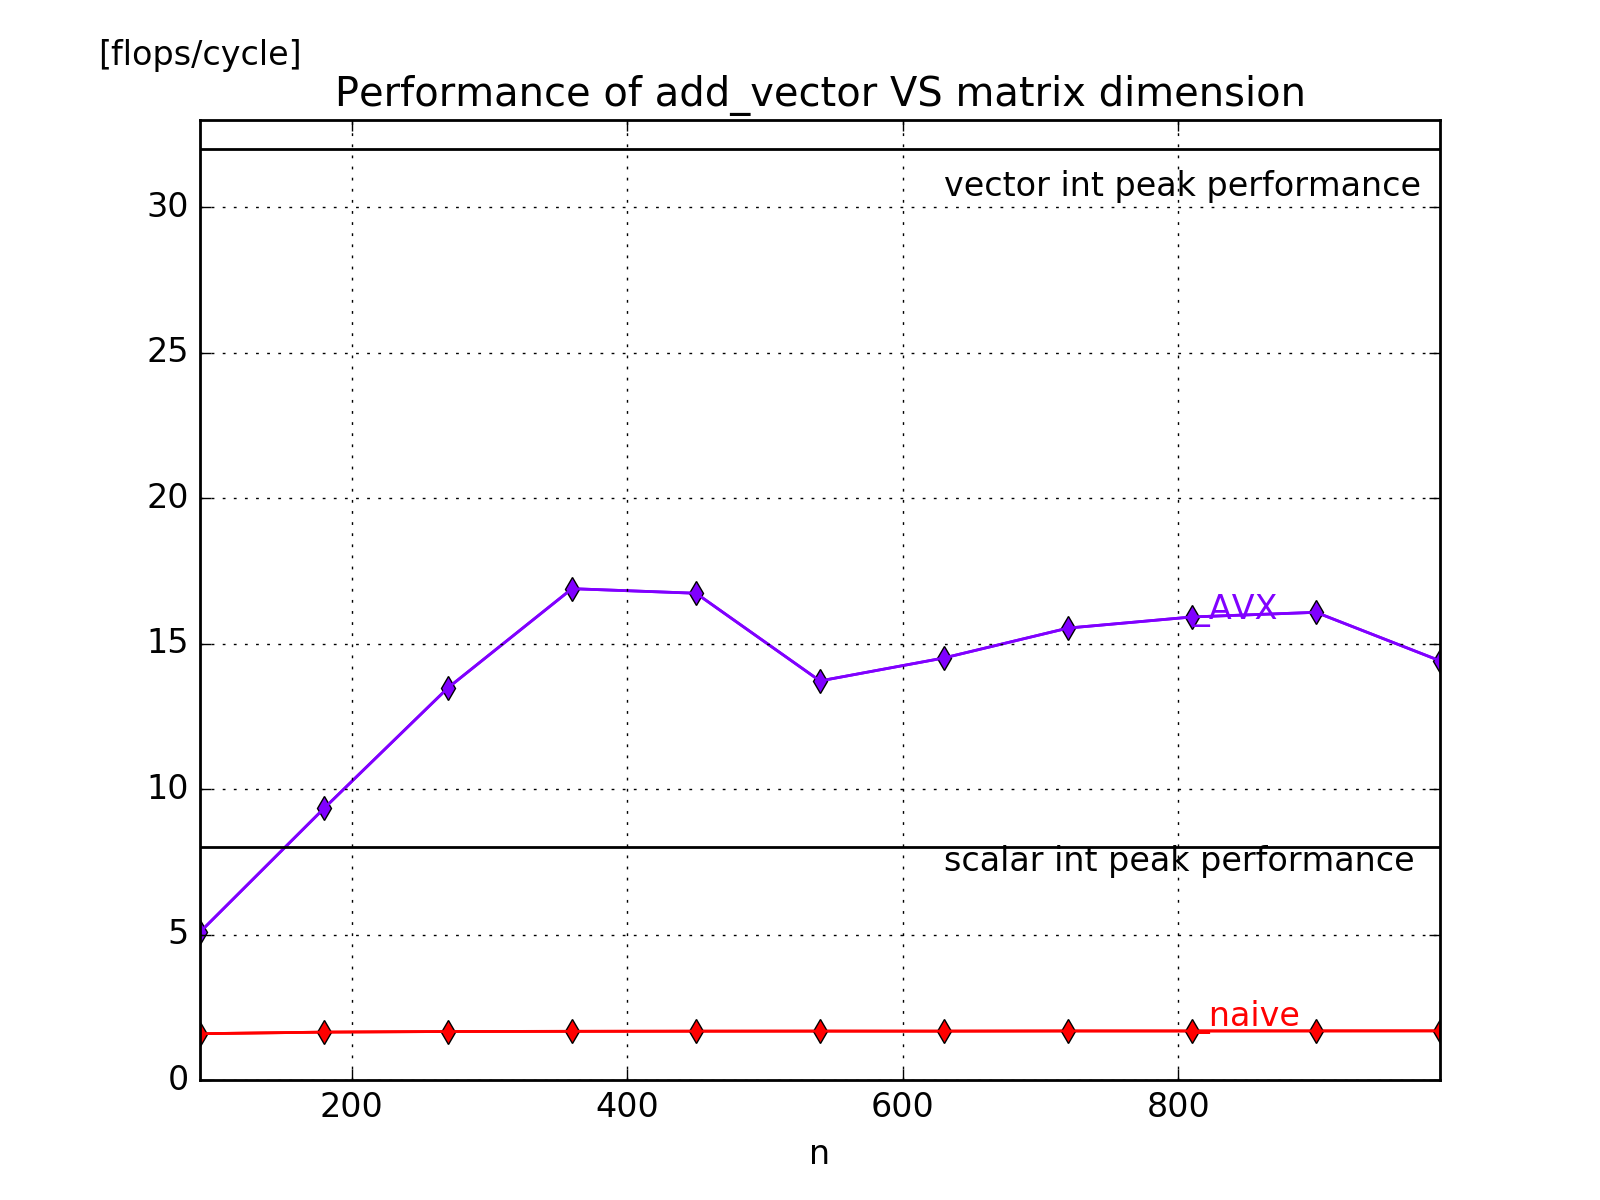
\includegraphics[width=0.5\textwidth]{Performance_add_vector.eps}
\caption{Performance plot of the function \emph{add\_vector}}
\label{figure:performance_add_vector}
\end{figure}

\begin{figure}[h]
	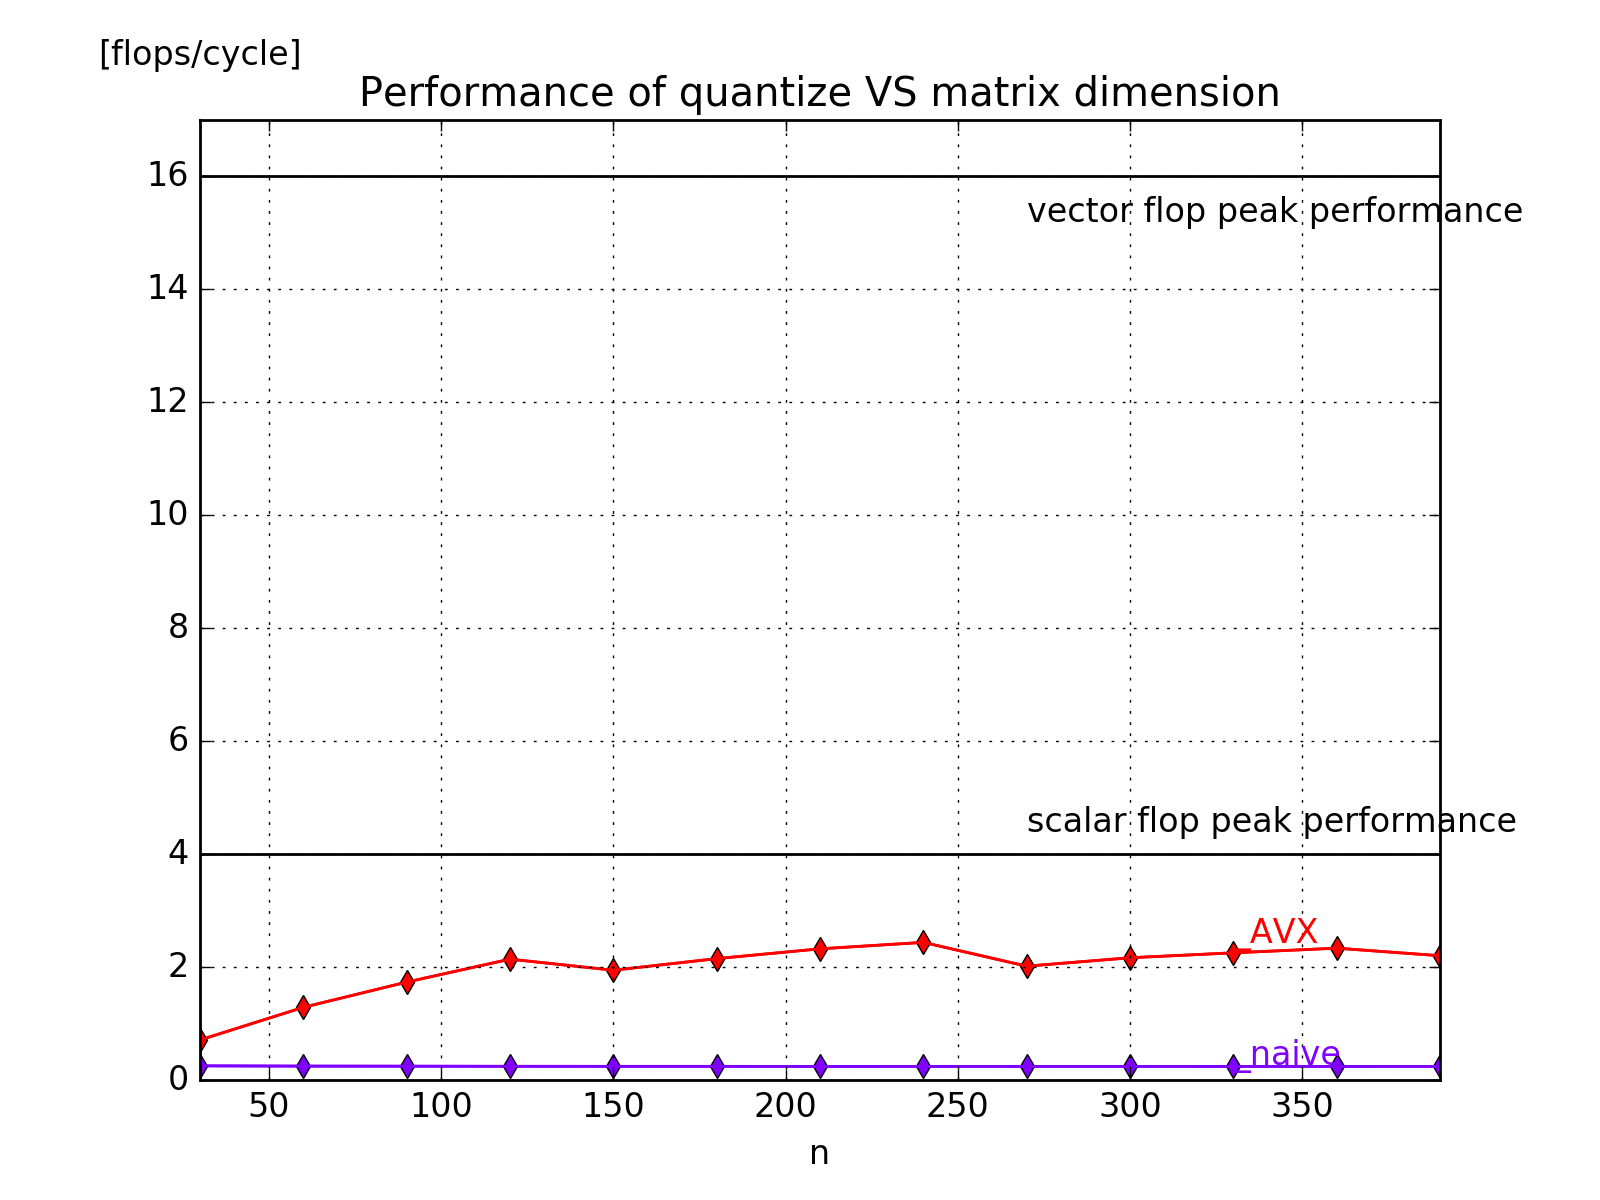
\includegraphics[width=0.5\textwidth]{Performance_quantize.eps}
	\caption{Performance plot of the function \emph{quantize}}
	\label{figure:performance_quantize}
\end{figure}

\begin{figure}[h]
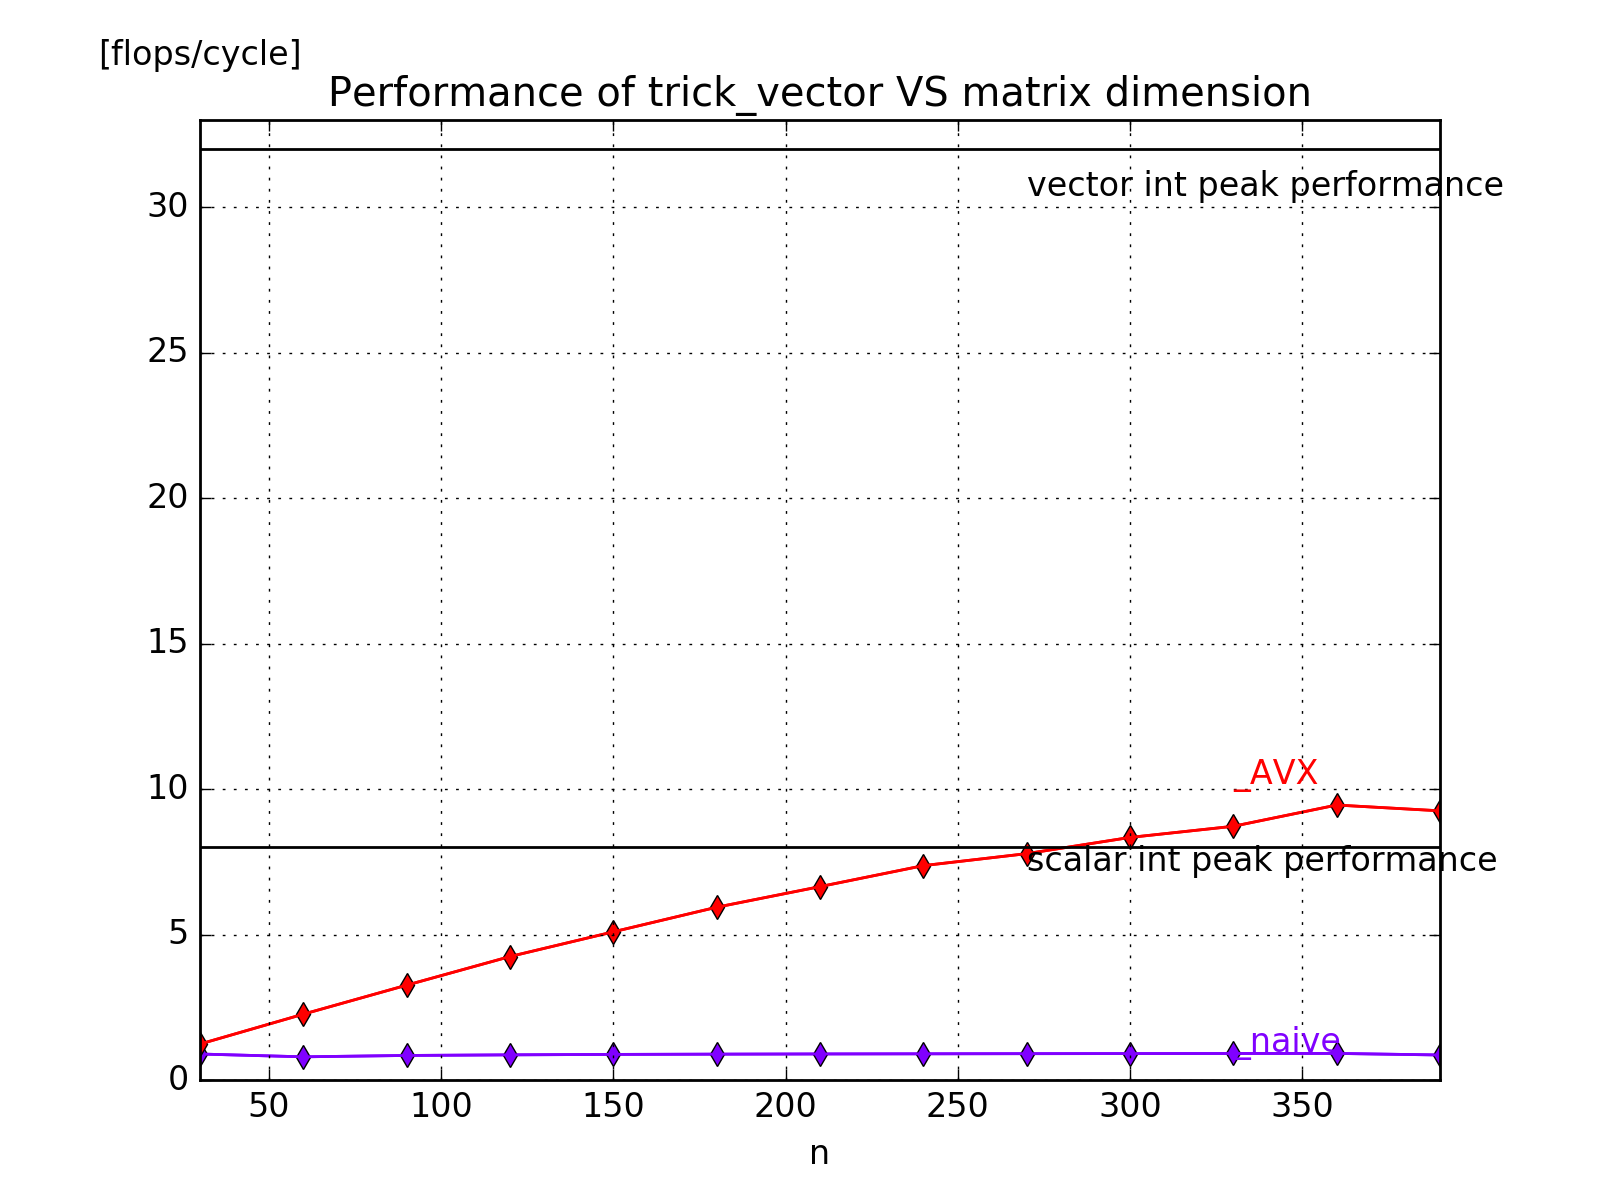
\includegraphics[width=0.5\textwidth]{Performance_trick_vector.eps}
\caption{Performance plot of the function \emph{trick\_vector}}
\label{figure:performance_trick_vector}
\end{figure}

\begin{figure}[h]
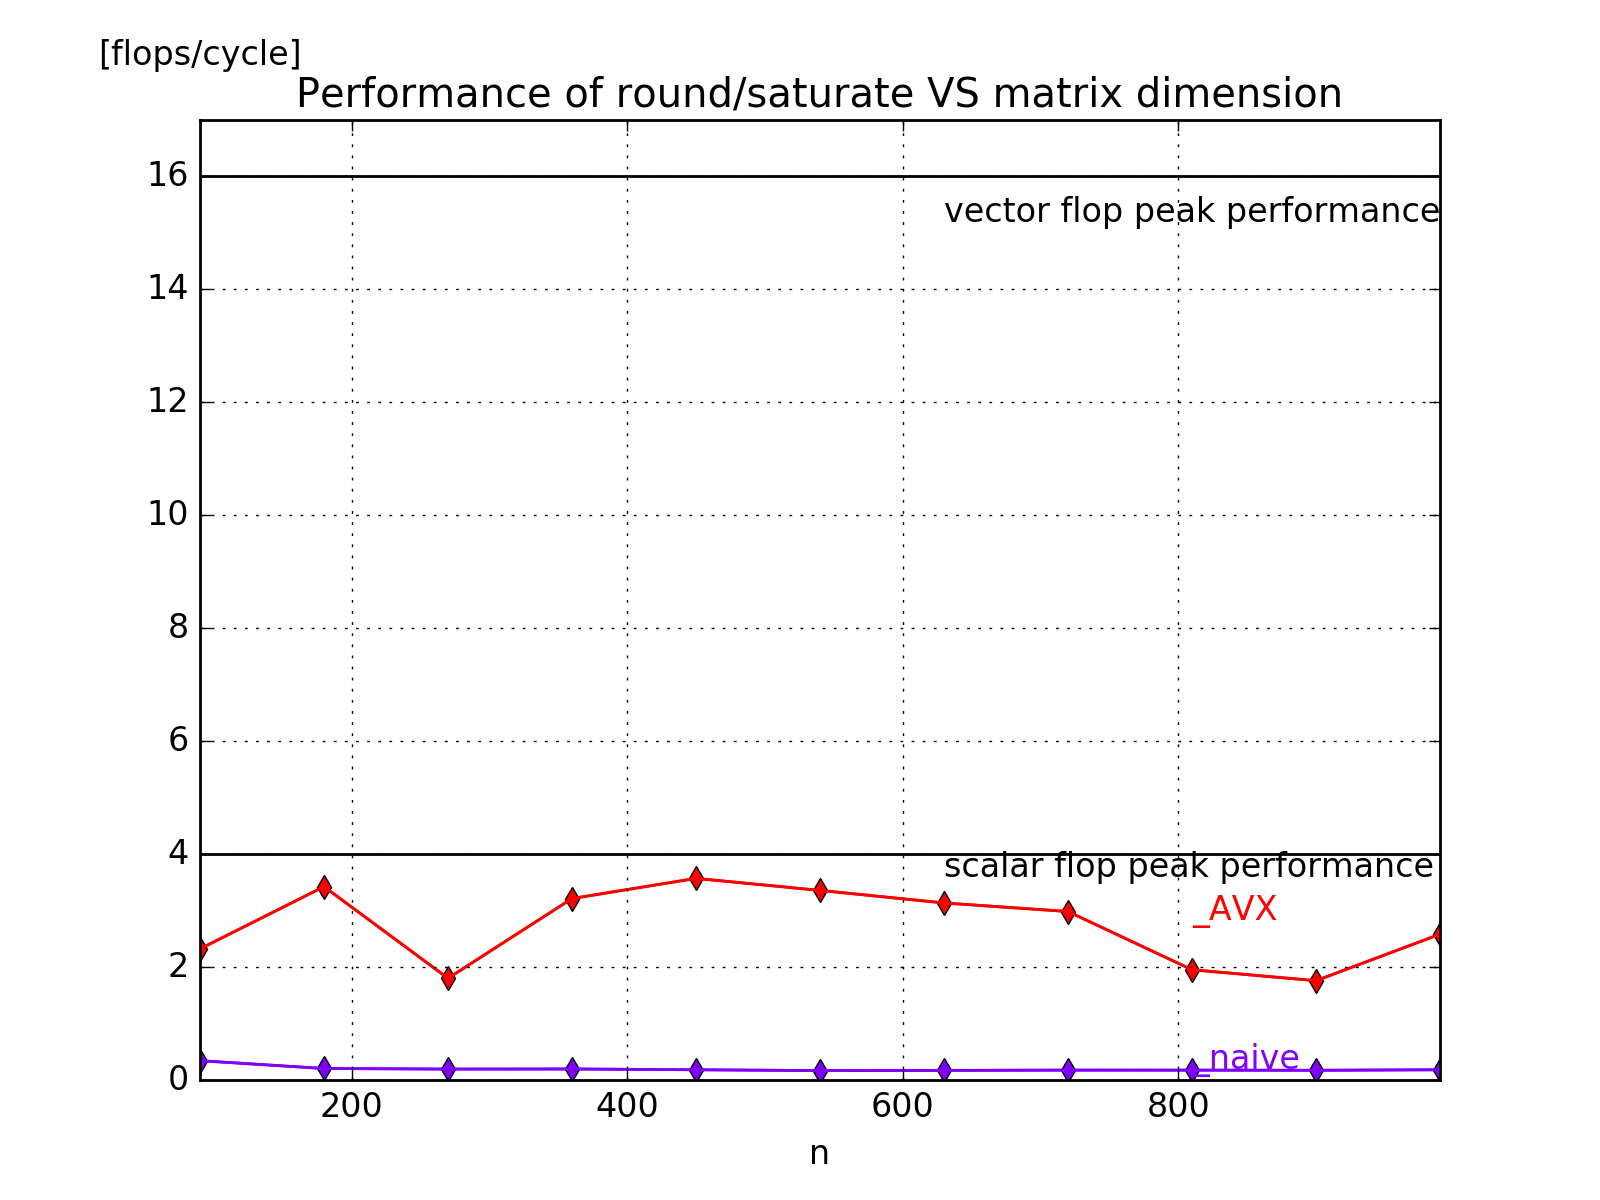
\includegraphics[width=0.5\textwidth]{Performance_round_saturation.eps}
\caption{Performance plot of the function \emph{round\_saturation}}
\label{figure:performance_round_saturation}
\end{figure}

The maximal gain in performance that the vectorization can allow for the functions \emph{trick\_vector} and \emph{add\_trick\_vector} is $16$X, that is the size of the accumulator vector for 16 bit integers. The measured performance gain are respectively  $9.8$X and $8.5$X.

\cref{figure:performance_quantize} and \cref{figure:performance_round_saturation} show the performance plot for the functions \emph{quantize} and \emph{round\_saturation}. The measured performance gain are respectively $9.2$X and $14.2$X. 

In \cref{figure:cycles_qmm_comparison} we can see the runtime plot for the whole pipeline. The implementation \emph{trick\_blocking\_AVX} is obtained combining the \emph{QMM\_kernel\_blocking} with the vectorized implementation of all the other sub-functions. The overall speedup is $2.5$X.
\section{Conclusions}
The experimental results presented in the previous sections outline
the benefits of performing vectorization and matrix blocking to achieve
a significant speedup over a naive implementation. The key ingredient in
the approach outlined above lies in the decision to map a tile of $2 \times 2$
floats to a single 16-bit integer (using a struct of 4 members with 4 reserved bits
respectively). Through this construction, the algorithms outlined in the previous are accessible
in a convenient form that lends itself to simply vectorize the load, quantize, round and saturate functions,
while also enabling a simplified blocking scheme for quantized matrix multiplication. More importantly,
each of the individual optimizations performed demonstrate the ability to improve over the current optimized
implementations of the General Matrix Multiplication with Low Precision library developed by Google. Although
this library is able to achieve overall better results due to the inclusion of auto-tuning approaches, it is possible
that through inclusion of our approaches, the store, load, quantization and subsequently the auto-tuning approaches could
achieve better overall results. On the other hand, the quantization process only needs to be performed once, and
it is not necessary for quantization to be performed on an embedded device, so the benefit of including the work performed
in this project is of minute importance in a general setting. 
%However, envisioning a scenario where devices
%with reduced memory capacity receive weights to neural networks from an external source (along with precomputed minimum
%and maximum values for each matrix). In such a scenario, the work done in this project would enable each of those devices to perform quantization
%locally and store the compressed weights as 4-bit integers and subsequently perform inference locally. This is particularly useful in a scenario where
%a distributed set of nodes are required to quantize weights to the neural network in different formats, and a central entity provides these weights
%as floating point numbers.
%
%Here you need to briefly summarize what you did and why this is
%important. {\em Do not take the abstract} and put it in the past
%tense. Remember, now the reader has (hopefully) read the paper, so it
%is a very different situation from the abstract. Try to highlight
%important results and say the things you really want to get across
%(e.g., the results show that we are within 2x of the optimal performance ... 
%Even though we only considered the DFT, our optimization
%techniques should be also applicable ....) You can also formulate next
%steps if you want. Be brief.



% References should be produced using the bibtex program from suitable
% BiBTeX files (here: bibl_conf). The IEEEbib.bst bibliography
% style file from IEEE produces unsorted bibliography list.
% -------------------------------------------------------------------------

\newpage
\bibliographystyle{IEEEbib}
\bibliography{HTWFNC_library.bib}

\end{document}

